% Copyright 2022 Thomas Ascher
% SPDX-License-Identifier: CC-BY-SA-4.0

\documentclass[a4paper,parskip=half]{scrartcl}

\usepackage[T1]{fontenc}
\usepackage{mathpazo}
%\usepackage[math]{iwona}
%\usepackage[math]{kurier}
%\usepackage{mathpazo}
\usepackage[naustrian]{babel}
\usepackage{csquotes}
%\usepackage{cmbright}
%\usepackage[regular,condensed,sfdefault]{roboto}
\usepackage{booktabs}
\usepackage{graphicx}
\usepackage{chemformula}
%\usepackage{euler}
%\usepackage{amsmath,amsfonts,amssymb}
\usepackage{icomma}
%\usepackage{textcomp}
\usepackage{gensymb}
%\usepackage{mathastext}
\usepackage{float}
\usepackage[style=apa,backend=biber]{biblatex}
\DeclareLanguageMapping{naustrian}{naustrian-apa}

\usepackage[hidelinks,pdfencoding=auto,
  pdfauthor={Thomas Ascher},
  pdfusetitle,
  pdfkeywords={Bier,Bitterung,Bitterstoffausbeute,IBU,Tinseth,Rager,Garetz}]{hyperref}
\usepackage{microtype}
%\DisableLigatures{encoding=*, family=*}

\setkomafont{disposition}{\normalfont\bfseries}

\addto\extrasnaustrian{
\def\figureautorefname{Abb.}
\def\tableautorefname{Tab.}
\def\equationautorefname{Gl.}
}

\addto\captionsnaustrian{
\renewcommand{\figurename}{Abb.}
\renewcommand{\tablename}{Tab.}
}

\NewBibliographyString{gethesis}
\DefineBibliographyStrings{naustrian}{
  mathesis = {Masterarbeit},
  gethesis = {Diplomarbeit},
}

\newcommand{\BA}{\mathit{BA}}
\newcommand{\BAKt}{{\mathit{BA}}_{\mathit{Kt}}}
\newcommand{\IBU}{\mathit{IBU}}
\newcommand{\umin}{\:[\textrm{min}]}
\newcommand{\uden}{\:[\text{g/cm³}]}
\newcommand{\uper}{\:[\text{\%}]}
\newcommand{\uli}{\:[\text{l}]}
\newcommand{\ume}{\:[\text{m}]}
\newcommand{\ucon}{\:[\text{mg/l}]}
\newcommand{\FKd}{F_{\mathit{Kd}}}
\newcommand{\FHR}{F_{\mathit{HR}}}
\newcommand{\FSP}{F_{\mathit{SP}}}
\newcommand{\FAH}{F_{\mathit{AH}}}
\newcommand{\FHF}{F_{\mathit{HF}}}
\newcommand{\FHS}{F_{\mathit{HS}}}
\newcommand{\FFil}{F_{\mathit{FI}}}
\newcommand{\dPfvw}{d_\mathit{Pfvw}}
\newcommand{\dKt}{\overline{d_{\mathit{Kt}}}}

\title{Eine bittere Angelegenheit: IBU Berechnungen}
\author{Thomas Ascher <thomas.ascher@gmx.at>}
\date{\today, \href{http://creativecommons.org/licenses/by-sa/4.0/}{CC BY-SA 4.0}}

\addbibresource{hopfenbittere.bib}

\begin{document}
\maketitle

\section*{Einleitung}

Hopfen, der auch als Seele des 

\parencite{Bastgen2020}
%TODO

Meiste Bittere vom Hopfen, ein Teil von Röstmalzen \parencite[11]{Garetz1994}

\parencite[10]{Garetz1994}
Aroma, Bittere und Haltbarkeit

\section*{International Bitterness Unit}

Die vorrangigen Bitterstoffe im Bier sind die Isomere der Alphasäuren des Hopfens: Isohumulone, Isocohumulone und Isoadhumulone. Darüber hinaus tragen auch noch weitere Hopfenbestandteile zum Bittereindruck bei, insbesondere Oxidationsprodukte der Alpha- und Betasäuren. \parencite{MEBAK2020}

Für die Bildung der Weichharze, zu denen Alpha- und Betasäuren (Lupulone, Colupulone und Adlupulone) zählen, sind die Lupulindrüsen in den Dolden der weiblichen Hopfenpflanzen zuständig. Nicht oxidierte Weichharze sind weder in Würze noch Bier bei Raumtemperatur gut lösbar. Die Alphasäuren unterlaufen jedoch während des Hopfenkochens einem Isomerisierungsprozess, einer molekularen strukturellen Veränderung, und bilden die Isoalphasäuren, welche in Lösung verbleiben. \parencite{Hall1997}

Die vorrangige Kennzahl zur Beschreibung des sensorischen Bittereindrucks eines Biers ist die International Bitterness Unit (IBU). Eine IBU entspricht einer Konzentration von einem Milligramm Isoalphasäure pro Liter Bier. Bei stark beziehungsweise kalt gehopften Bieren lässt sich der sensorische Bittereindruck durch vermehrt eingebrachte oxidierte Hopfenbestandteile und Polyphenole nicht mehr ausreichend durch die IBU charakterisieren. Die Schaffung neuer Wahrnehmungsmodelle, die unter anderem neben den Isoalphasäurekonzentration auch Oxidationsprodukte und den Alkoholgehalt berücksichtigen, sind Gegenstand  aktueller Forschung. \parencite{Kishimoto2021}

Von den normgebenden Gremien der Brauindsutrie – der \href{https://www.asbcnet.org}{ASBC}, der \href{https://europeanbreweryconvention.eu}{EBC} und später auch der \href{https://www.mebak.org}{MEBAK} – wurden zur Messung der IBU ein in den 1950er-Jahren definiertes,  kostengünstiges, spektralphotometrisches analytisches Verfahren ratifiziert. Dabei erfolgt keine direkte Messung des Isoalphasäurekonzentration, sondern eine Korrelation der gemessenen Lichtabsorption einer aufbereiteten Bierprobe bei einer Wellenlänge von 275~nm. Es absorbieren aber auch andere Bestandteile der Probe Licht in diesem Spektrum. Die angewendete Korrelation, die Multiplikation des Messwertes mit 50, ist allerdings nur für typische Biere der 1950er und 1960er-Jahre gültig. \parencites{ASBC2011}{Hosom2017}

\parencite[5\psq]{Malowicki2005}
Overlap zwischen verschiedenen Inhaltsstoffen. Photemeter outdated HPLC Messung 

Die Anschaffungskosten für Spektralphotometer und HPLC-Apparaturen sind für Privatpersonen nur schwer zu decken. \textcite{Calado2019} haben aber eine kostengünstige, auf Fluoreszenz basierte, Messmethode unter dem Einsatz einer UV-LED, einer Digitalkamera und Bildverarbeitungsalgorithmen vorgeschlagen, die eine mittlere quadratische Abweichungen von 3~IBU im Vergleich zur Messung mit einem Spektralphotometer erreicht. Darüber hinaus bieten einige Labore, wie „\href{https://bieranalyse.de}{Bieranalyse Fuchs}“ und „\href{https://www.weinlabor-krauss.de}{Weinlabor Krauß}“, bezahlbare Messdienste für Heimbrauer/-innen an.

%TODO IBU limit

\section*{Bitterstoffausbeute}

Nur etwa 10 bis 40~\% der dosierten Alphasäuremenge gelangt als Isoalphasäure in das fertige Bier. Der genaue Prozentsatz ist dabei unter anderem abhängig wie viel Alphasäure aus dem eingesetzten Hopfenprodukt extrahiert werden kann, wie vollständig die Isomerisierung verläuft und wie viele Bitterstoffe durch Trubbildung, Filterung und Gärung verloren gehen. \parencite[9]{Malowicki2005}

Der Prozessparameter, der beschreibt wie effektiv Bitterstoffe verwertet werden, heißt Bitterstoffausbeute (BA) und ist gemäß \autoref{eq:badef} basierend auf dem Verhältnis zwischen den in einem Bier enthaltenen Bittereinheiten und der in der Pfannenvollwürze (Pfvw) dosierten Alphasäure definiert. Die Bitterstoffausbeute lässt sich alternativ auch in Bezug auf die Anstellwürze statt dem fertigen Bier spezifizieren. Dabei sind aber keine Gärungsverluste berücksichtigt. \parencite[163]{Annemueller2015} 

\begin{equation}
\BA \uper = \frac{\text{Isohumulongehalt des Bieres [IBU]}}{\text{Alphasäuredosage in kalter Pfvw} \ucon} \cdot 100
\label{eq:badef}
\end{equation}

Sind die Bitterstoffausbeute und der Alphasäuregehalt eines Hopfens bekannt, so kann für eine Hopfengabe die resultierenden Bittereinheiten durch \autoref{eq:ibucalc} bestimmen werden \parencite{Thesseling2019}.
%TODO messung per ballen

\begin{equation}
\IBU = \frac{\text{Hopfenmenge [mg]} \cdot \frac{\text{Alphasäuregehalt} \uper}{100} \cdot \frac{\BA}{100}}{\text{Volumen kalte Anstellwürze} \uli}
\label{eq:ibucalc}
\end{equation}

Folgende Faktoren begünstigen die BA: längere Kochzeiten,
höhere Kochtemperaturen, höherer Zerkleinerungsgrad des Hopfens, geringere Alphasäuredosierung, geringerer Extraktgehalt in der Würze, geringere Trubbildung und schnellere Ausflockung der Hefe \parencite{Hosom2017}. Kochzeiten zwischen 60 bis 90~Minuten (\autoref{fig:utiltinseth}) sind in Hinsicht auf die Hopfenausnutzung optimal \parencite[5]{Malowicki2005}. Dabei ist jedoch zu beachten, dass mit zunehmender Kochdauer Isoalphasäuren zu anderen, teilweise sensorisch unangenehmen, Produkten abgebaut werden \parencite{Kappler2010}.

\begin{figure}[H]
\centering
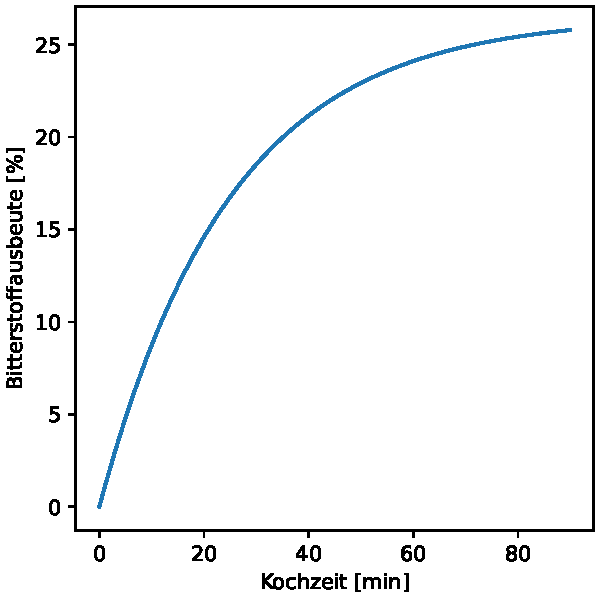
\includegraphics[width=6cm]{graph_tinseth.pdf}
\caption{Bitterstoffausbeute nach Tinseth (Ascher, 2022)}
\label{fig:utiltinseth}
\end{figure}

Während der Gärung treibt die gebildete Kohlensäure einen Teil der Isoalphasäuren aus. Ein Teil davon verfängt sich in der Hefedecke oder sammelt sich am Rand des Gärbehälters und verhärtet sich aufgrund der Oxidierung. Ein weiterer Teil haftet an den Hefezellen an. Je langsamer eine Hefe ausflockt, desto mehr Bitterstoffe können an ihr anhaften und sendimentieren. Verbleibt die Hefe im Bier so wie beim Weißbier, ist dementsprechend auch der Bitterstoffverlust geringer. \parencite[126]{Garetz1994} 

\section*{Hopfenprodukte und Hopfengaben}

Dolden werden nach der Ernte aufgrund ihrer Verderblichkeit zunächst getrocknet, konditioniert, gepresst und schließend zu verschiedenen Endprodukten weiterverarbeitet. Ausgenommen davon ist der Grünhopfen, dessen Verwendung möglichst direkt nach der Ernte erfolgt. Eine Erhebung des Alphasäuregehalts des Grünhopfens erfolgt im Normalfall nicht. Im Heimbraubereich sind vor allem T90 Pellets, die circa aus 95~\% des ursprünglichen Pflanzenmaterials bestehen, gängig. Bei deren Herstellung werden Dolden zunächst geschreddert, gepresst und extrudiert. Das Schreddern zerstört auch die Lupulindrüsen, was beim Hopfenkochen für eine bessere Ausbeute sorgt. Wird bis zu 45~\% des ursprünglichen Pflanzenmaterials entfernt, entstehen dabei die angereicherten T45 Pellets. Es ist möglich bei der Verarbeitung noch weiteres Pflanzenmaterial zu entfernen und somit konzentriertes Lupulinpulver zu erhalten. Dieses Endprodukt wird zum Beispiel unter den Namen Cryo Hops, Hop Hash oder Nectar vertrieben. Alternativ können Hopfenharze auch durch verschiedene Lösungsmittel aus den Dolden gelöst werden. Einige Hopfenprodukte sind auch in vorisomerisierter Form erhältlich.
\parencites[166-172]{Nottebohm2020}[80-90]{Garetz1994}


\parencite[58]{Hall1997}
Schätzung alle Effekte für Bitterstoffausbeute zu beachten schwierig
Starke Schwankungen bei Doldenhopfen
geringer bei Pellets weil geblendet
kommerzielle brauereien können messen und batches blenden.


 Darüber hinaus erfolgt auch unter einer Temperatur von 90~°C eine substantielle Isomerisierung \parencite[29]{Malowicki2005}.

\section*{Effekte der Hopfenalterung}

Nördliche Hemisphere einmal Ernte pro Jahr. Mitte August bis
Anfang September.
\parencite[97]{Garetz1994}

\parencite[97]{Garetz1994} Hopfen verliert Alphasäure und Öle
durch Oxidation. Vakuimieren und gekühlte Aufbewahrung verlangsamen
den Prozess. Auch kein Licht. 

\parencite[103]{Garetz1994} Alphasäure oxidiert an luft, oxidationsprodukte
nicht mehr isomerisierbar. Nicht mehr so bitter. Betssäuren bilden
Bitterstoffe. bei Oxidation.

\parencite[104]{Garetz1994} 
Unter gleichen Lagerbedingungen verlieren Hopfen unterschiedlich an
Alpha wegen unterschiedliche Menge Oxidantien.
-HSI spektroskopisch analyse von alpha und beta. Test für Halbarkeit:
Verlust von Alpha und Betasäure über 6 Montate über Raumtemperatur 20c.
Korrelation zwischen beiden. Der ursprüngliche Alphagehalt und der
zkünftige
Ölverluste nicht ausreichend erforscht.

\parencite[104]{Garetz1994} 
HSI Nummer, nich von Händlern, hauptsächlich als interne Referenz
in den Laboren
Percent Alpha remaining or Lost after 6 Months at 20c
\% Alpha /nach 6 Monaten



\parencite[52]{Davidson1997}
Oxidation von beta säuren -> ähnliche hulupones wie isohomulone


% TODO ev. Berechnung beschreiben
% TODO Diagramm zu Alphaverlust

\section*{Modelle zur Schätzung der Bitterstoffausbeute}

Spätenstens seit der Veröffentlichung des Berechnungsverfahrens nach
Rager im Zymurgy Magazin im Jahr 1990 stand einem breiteren
Publikum die Möglichkeit zur Verfügung, Berechnungen für Hopfengaben auf
Basis der IBU
durchzuführen \parencite[59]{Hall1997}. Im Verlauf der Neunzingerjahre
sind dann noch weitere Modelle zur Schätzung der Bitterstoffausbeute entstanden.
Von diesen hat sich das Tinseth Modell inzwischen als De-facto-Standard im
Heimbraubereich etabliert \parencite[185]{Hieronymus2012}.

Die Umgestaltung bestehender und die Schaffung neuer Bierstile
durch die Craft Beer Szene in den letzten zwanzig Jahren hat auch zu Änderungen
der Abläufe bei Hopfengaben, in der Form der vermehrten Anwendung von Vorderwürze-
und Whirlpoolhopfung, geführt. Die Modelle der Neunzigerjahre sind aber
nicht dafür ausgelegt, große Hopfengaben gegen Ende des Kochprozesses korrekt
zu berücksichtigen. Aktuelle Ansätze versuchen diesen Fehler zu korrigieren.
\parencite[39]{Novotny2018}


\parencite[51]{Holle2010}
ibu = mg hop * util * alpha acid \% / l

\parencite[127]{Garetz1994} 
Keine in professioneller Brauliteratur, Messtechnisch erhoben
werden. Nach einigen Brauversuchen lässt sich also einstellen.
Blending mehrer Batches.

\parencite[76]{Daniels1996}
Große Brauereien können große Hopfenmengen mischen und
Biere um unterschiede auszugleichen.

\parencite[51]{Holle2010}
Einziger verlässliche Weg ist labortechnische Analysen.




\subsection*{Historische Modelle}

Hall hat einen Großteil der relevanten, ab 1990 veröffentlichten, Modelle analysiert,
deren Daten normalisiert und in ein gemeinsames Berechnungsschema überführt. Dabei ist
pro Hopfengabe zuerst eine initiale Bitterstoffausbeute basierend auf der Kochzeit
($\BAKt$) zu bestimmen und anschließend durch mehrere Korrekturfaktoren anzupassen.
Aus den eingebrachten Alphasäuremengen der einzelnen Gaben und den ermittelten
Bitterstoffausbeute lässt sich dann ein IBU Wert für ein Rezept berechnen. \parencite[59-65]{Hall1997}

% TODO verweis konzentration

Folgende Korrekturfaktoren sind modellabhängig vorgesehen:

\begin{itemize}
\item Relative Dichte der „Kochwürze“ ($\FKd$)
\item Hopfenrate ($\FHR$)
\item Siedepunkt des Wassers basierend auf der Seehöhe ($\FSP$)
\item Sedimentationsverhalten der Hefe ($\FAH$)
\item Hopfenform: Dolden oder Pellets ($\FHF$)
\item Verwendung eines Hopfensacks ($\FHS$)
\item Filtration ($\FFil$)
\end{itemize}

Die Umrechnung von Extraktgehalt in relative Dichte erfolgt auf Basis
der Plato Tabellen über die Goldiner Gleichungen (\autoref{eq:calcptosg})
oder vergleichbaren Näherungsverfahren \parencite[140\psq]{Spedding2016}.

\begin{equation}
d_{\frac{20}{20}} \uden = \frac{\degree P}{258,6 - \degree P / 258,2 \cdot 227,1} + 1
\label{eq:calcptosg}
\end{equation}

\subsubsection*{Burch (1986)}

In der ersten Ausgabe des Buches, basierend auf kommerziellen erfahrungswerten \parencite[28-32]{Burch1992}

Auch für Dry hop 5 \parencite[33]{Burch1992}

\begin{table}[H]
\centering
\begin{tabular}{rr}
\toprule
\multicolumn{1}{c}{\textbf{Kochzeit [min]}} & \multicolumn{1}{c}{\textbf{Ausbeute [\%]}} \\
\midrule
0–14  & 5 \\
15–40 & 8–12 \\
45–60 & 28–30 \\
\bottomrule
\end{tabular}
\caption{Bitterstoffausbeute für Dolden nach Burch \parencite[33]{Burch1992}}
\label{table:burchbakt}
\end{table}

\subsubsection*{Rager (1990)}

Die Grundlage für Ragers Modell bildeten Heimbraubücher von Fred Eckhardt,
Dave Miller und Byron Burch. Er hat die darin enthaltenen Informationen
zu einem Berechnungsverfahren zusammengeführt \parencite[53]{Rager1990}. 
Garetz kritisierte an Ragers Methode, dass nur der Korrekturfaktor
$\FKd$ berücksichtigt wurde \parencite[134]{Garetz1994}.

Für die Modellberechnung ist zuerst die Ausbeute $\BAKt$ über die \autoref{table:ragerbakt}
oder die \autoref{eq:ragerbakt} auf Basis der Kochdauer der jeweiligen Hopfengabe
zu wählen \parencite{Steinmeyer2021}.
Danach ist der Korrekturfaktor $\FKd$ anhand der relativen Dichte der
Pfannenvollwürze ($\dPfvw$) gemäß \autoref{eq:ragerga} und \autoref{eq:ragerfkd}
zu bestimmen \parencite[53]{Rager1990}.
Abschließend erfolgt die Berechnung der Bitterstoffausbeute über \autoref{eq:ragerba}.

\begin{table}[H]
\centering
\begin{tabular}{rr}
\toprule
\multicolumn{1}{c}{\textbf{Kochzeit [min]}} & \multicolumn{1}{c}{\textbf{Ausbeute [\%]}} \\
\midrule
0–5             & 5 \\
6–10            & 6 \\
11–15           & 8 \\
16–20           & 10,1 \\
21–25           & 12,1 \\
26–30           & 15,3 \\
31–35           & 18,8 \\
36–40           & 22,8 \\
41–45           & 26,9 \\
46–50           & 28,1 \\
51–60           & 30 \\
\bottomrule
\end{tabular}
\caption{Bitterstoffausbeute für Dolden nach Rager \parencite[54]{Rager1990}}
\label{table:ragerbakt}
\end{table}

\begin{equation}
\BAKt \uper = 18,11 + \left(13,86 \cdot \tanh{\frac{\text{Kochzeit} \umin - 31,32}{18,27}}\right)
\label{eq:ragerbakt}
\end{equation}


\begin{equation}
\mathit{DA} = \begin{cases}
0 \quad \text{für} \quad d_{\mathit{Pfvw}} \le 1,050 \uden, \\
\frac{d_{\mathit{Pfvw}} - 0,05}{0,2} \quad \text{für} \quad d_{\mathit{Pfvw}} > 1,050 \uden.
\end{cases}
\label{eq:ragerga}
\end{equation}

\begin{equation}
\FKd = \frac{1}{1 + \mathit{DA}}
\label{eq:ragerfkd}
\end{equation}


\begin{equation}
\BA \uper = \BAKt \cdot \FKd
\label{eq:ragerba}
\end{equation}

\subsubsection*{Garetz (1994)}

Das grundlegende Berechnungsverfahren für das von Garetz in 1994
veröffentlichte Modell übernahm er von Rager. Anpassungen sind jedoch an
der Tabelle zur Bestimmung der Ausbeute anhand der Kochzeit und den
Korekturfaktoren erfolgt \parencite[134-144]{Garetz1994}.

Die Berechnung nach Garetz kann in mehreren Ausbaustufen erfolgen,
deren Umfang von den gewählten Korrekturfaktoren abhängt.
Der Minimalumfang ist dabei durch \autoref{eq:garetzba1} definiert
\parencite[137]{Garetz1994}.
Zunächst ist die Ausbeute $\BAKt$ anhand der Kochzeit der jeweiligen 
Hopfengabe über die \autoref{table:garetzbakt} oder die \autoref{eq:garetzbakt} zu bestimmen \parencite{Steinmeyer2021}. Danach erfolgt die
Berechnung der Faktoren $\FKd$, $\FHR$ und $\FSP$ gemäß
\autoref{eq:garetzkd}, \autoref{eq:garetzhr} und \autoref{eq:garetzsp}.
Der Faktor $\FHR$ basiert auf dem Zielwert der gesamten Bittereinheiten
eines Rezepts. Das Modell von Garetz geht nämlich im Standardfalls
davon aus, Hopfenmengen auf Basis gewünschter IBU Werte zu schätzen.
Hier ist es entweder möglich den Faktor zunächst zu ignorieren und
und iterativ den Gesamtwert zu schätzen oder den Faktor bei nur
einer Hopfengabe durch eine quadratische Gleichung zu eliminieren      \parencite[63]{Hall1997}.

\begin{table}[H]
\centering
\begin{tabular}{rr}
\toprule
\multicolumn{1}{c}{\textbf{Kochzeit [min]}} & \multicolumn{1}{c}{\textbf{Ausbeute [\%]}} \\
\midrule
0–10            & 0 \\
11–15           & 2 \\
16–20           & 5 \\
21–25           & 8 \\
26–30           & 11 \\
31–35           & 14 \\
36–40           & 16 \\
41–45           & 18 \\
46–50           & 19 \\
51–60           & 20 \\
61–70           & 21 \\
70–80           & 22 \\
81–90           & 23 \\
\bottomrule
\end{tabular}
\caption{Bitterstoffausbeute für Dolden nach Garetz \parencite[138]{Garetz1994}}
\label{table:garetzbakt}
\end{table}

\begin{equation}
\BAKt \uper = 7,2994 + \left(15,0746 \cdot \tanh{\frac{\text{Kochzeit} \umin - 21,86}{24,71}}\right)
\label{eq:garetzbakt}
\end{equation}


\begin{equation}
\mathit{CF} = \begin{cases}
1 \quad \text{bei keiner Verdünnung der Kaltwürzemenge}, \\
\frac{\text{Kaltwürzemenge} \uli}{\text{Pfannevollmenge} \uli} \quad \text{bei Verdünnung der Kaltwürzemenge}.
\end{cases}
\label{eq:garetzcf}
\end{equation}

\begin{equation}
d \uden = \begin{cases}
\dPfvw \quad \text{für} \quad \mathit{CF} = 1, \\
\left( \left( \dPfvw - 1 \right) \cdot \mathit{CF} \right) + 1 \quad \text{für} \quad \mathit{CF} \ne 1.
\end{cases}
\label{eq:garetzbg}
\end{equation}

\begin{equation}
\mathit{DA} = \begin{cases}
0 \quad \text{für} \quad d \le 1,050 \uden, \\
\frac{d - 0,05}{0,2} \quad \text{für} \quad d > 1,050 \uden.
\end{cases}
\label{eq:garetzga}
\end{equation}

\begin{equation}
\FKd = \frac{1}{1 + DA}
\label{eq:garetzkd}
\end{equation}

\begin{equation}
\FHR = \frac{1}{\left( \frac{\text{IBU Rezept}}{260} \cdot \mathit{CF} \right) + 1}
\label{eq:garetzhr}
\end{equation}

\begin{equation}
\FSP = \frac{1}{\left(\frac{\text{Seehöhe} \ume \cdot 3,2808}{550} \cdot 0,02 \right) + 1}
\label{eq:garetzsp}
\end{equation}

\begin{equation}
\BA_1 \uper = \BAKt \cdot \FKd \cdot \FHR \cdot \FSP
\label{eq:garetzba1}
\end{equation}

Alle weiteren Faktoren erachtet Garetz als optional. Der Faktor
$\FAH$ (\autoref{eq:garetzah}) ist anhand des Sedimentationsverhaltens
der Hefe zu wählen. Je schneller eine Hefe sedimentiert, desto
weniger Isoalphasäure haftet an den Zellwenden an und desto
mehr Isoalphasäure bleibt in Lösung. Dementsprechend ist die
Bitterstoffausbeute um 5~\% nach unten oder nach oben zu korrigieren. 
Für Weißbier veranschlagt Garetz eine 20~\% höhere Ausbeute,
da die Hefe beim Trinken ebenfalls konsumiert wird.
Bei der Verwendung von Pellets erfolgt eine erhöhung der
Ausbeute um 10~\% bei einer Kochzeit bis 30~Minuten (\autoref{eq:garetzhf}).
Für Hopfensäcke ist eine Reduktion der Ausbeute,
basierend auf Packdichte, um bis zu 20~\% durchzuführen.
(\autoref{eq:garetzhs}). Der Einsatz eines Filtersystems kann
die Ausbeute inetwa um 1,25 bis 2,5~\% reduzieren (\autoref{eq:garetzfil}),
dementsprechend empfieht Garetz eine messtechnische Erhebung des Faktors $\FFil$. \parencite[140\psq]{Garetz1994}

\begin{equation}
\FAH = \begin{cases}
1,00 \quad \text{für normal sedimentierender Hefe}, \\
1,05 \quad \text{für schnell sedimentierender Hefe}, \\
0,95 \quad \text{für langsam sedimentierender Hefe}, \\
1,20 \quad \text{für Weißbierhefe}. \\
\end{cases}
\label{eq:garetzah}
\end{equation}


\begin{equation}
\FHF = \begin{cases}
1,0 \quad \text{für Dolden}, \\
1,1 \quad \text{für Pellets für} \quad 10 < \text{Kochzeit} \umin \le 30. \\
\end{cases}
\label{eq:garetzhf}
\end{equation}

\begin{equation}
\FHS = \begin{cases}
1,0 \quad \text{ohne Hopfensack}, \\
0,9 \quad \text{für lose gepackten Hopfensack}, \\
0,8 \quad \text{für dicht gepackten Hopfensack}. \\
\end{cases}
\label{eq:garetzhs}
\end{equation}

\begin{equation}
\FFil := \left[0,975, 0,9875 \right]
\label{eq:garetzfil}
\end{equation}

\begin{equation}
\BA_2 \uper = BA_1 \cdot \FAH \cdot \FHF \cdot \FHS \cdot \FFil
\label{eq:garetzba2}
\end{equation}

\subsubsection*{Mosher (1994)}

Bereits am Ende der Achzigerjahre hatte Mosher einen aus mehreren
Drehscheiben bestehenden Rechenschieber zur IBU Berechnung erstellt und später
auch vertrieben \parencite{Mosher2022}. Sein in 1994 veröffentlichtes
Buch „\citetitle{Mosher1994}“ enthält zwei Diagramme zur grafischen
Bestimmung der Bitterstoffausbeute für Kochzeiten bis zu drei Stunden
\parencite[160\psq]{Mosher1994}. Holle und \citeauthor{Thesseling2019} verwenden
einen Teil der abgemessenen Diagrammdaten noch immer in aktuelleren
Publikationen für grobe Abschätzungen \parencites[51]{Holle2010}{Thesseling2019}.

Die Bitterstoffausbeute nach Mosher ist basierend auf der relativen Dichte und
der Kochzeit der jeweiligen Hopfengabe zu bestimmen. Für Dolden ist
dabei der Wert aus \autoref{table:mosherbakt} und für Pellets aus
\autoref{table:mosherbaktpellets} zu entnehmen. Ob sich die
relativen Dichte dabei wie bei Rager auf die Pfannenvollwürze bezieht, ist aus Moshers Publikation nicht ersichtlich. Holle geht bei seinen Beispielen
von der Stammwürze aus \parencite[53]{Holle2010}.

\begin{table}[H]
\centering
\begin{tabular}{rrrrrrrr} 
\toprule
\multicolumn{1}{c}{\textbf{Kochzeit [min]}} & \multicolumn{7}{c}{\textbf{Ausbeute [\%]}}  \\
Relative Dichte [g/cm³]:                                        & 1,030 & 1,040 & 1,050 & 1,060 & 1,070 & 1,080  & 1,090                   \\
Extraktgehalt [\%w/w]:                                            & 7,6 & 10 & 12,4 & 14,7 & 17,1 & 19,3  & 21,6                   \\                                            
\midrule

5                                            & 5     & 5     & 4     & 4     & 3     & 3      & 3                          \\
15                                           & 12    & 12    & 11    & 11    & 11    & 10     & 9                          \\
30                                           & 17    & 17    & 16    & 16    & 15    & 15     & 13                         \\
45                                           & 21    & 21    & 20    & 19    & 18    & 17     & 16                         \\
60                                           & 24    & 23    & 23    & 22    & 21    & 20     & 18                         \\
90                                           & 28    & 27    & 26    & 26    & 25    & 23     & 21                         \\
\bottomrule
\end{tabular}
\caption{Bitterstoffausbeute für Dolden nach \citeauthor{Mosher1994} \parencite[51]{Holle2010}}
\label{table:mosherbakt}
\end{table}

\begin{table}[H]
\centering
\begin{tabular}{rrrrrrrr} 
\toprule
\multicolumn{1}{c}{\textbf{Kochzeit [min]}} & \multicolumn{7}{c}{\textbf{Ausbeute [\%]}}  \\
Relative Dichte [g/cm³]:                                        & 1,030 & 1,040 & 1,050 & 1,060 & 1,070 & 1,080  & 1,090                   \\
Extraktgehalt [\%w/w]:                                            & 7,6 & 10 & 12,4 & 14,7 & 17,1 & 19,3  & 21,6                   \\  
\midrule
5                                            & 6     & 6     & 5     & 5     & 4     & 4      & 3                          \\
15                                           & 15    & 15    & 14    & 14    & 13    & 13     & 11                         \\
30                                           & 22    & 21    & 21    & 20    & 19    & 18     & 16                         \\
45                                           & 26    & 26    & 25    & 24    & 23    & 22     & 21                         \\
60                                           & 29    & 28    & 28    & 27    & 26    & 25     & 23                         \\
90                                           & 35    & 34    & 33    & 32    & 31    & 29     & 27                         \\
\bottomrule
\end{tabular}
\caption{Bitterstoffausbeute für Pellets nach \citeauthor{Mosher1994} \parencite[51]{Holle2010}}
\label{table:mosherbaktpellets}
\end{table}

\subsubsection*{Daniels (1996)}

Das Modell von Daniels verwendet Teile der Berechnungsvorschriften
von Rager und Garetz aber eigene Tabellen für die Bestimmung
der Bitterstoffausbeute basierend auf der Kochzeit und des
verwendeten Hopfenprodukts (\autoref{table:danielsbakt} und \autoref{table:danielsbaktpellets}).
Der Faktor $\FKd$ ist nach Rager mit \autoref{eq:ragerfkd} zu berechnen.
Für den Faktor $\FHR$ hat Daniels eine eigene Tabelle vorgesehen,
die hier nicht angeführt wurde, nachdem deren Berechnung auch durch
\autoref{eq:garetzhr} möglich ist.
Die gesamte Bitterstoffausbeute wird gemäß \autoref{eq:danielsba} gebildet.
Neben Moshers Rechenschieber bilden noch weitere Quellen und eigene
Tests die Datenbasis für Daniels Tabellen. \parencite[80,85-88]{Daniels1996}

\begin{table}[H]
\centering
\begin{tabular}{rr}
\toprule
\multicolumn{1}{c}{\textbf{Kochzeit [min]}} & \multicolumn{1}{c}{\textbf{Ausbeute [\%]}} \\
\midrule
0–9            & 5  \\
10–19          & 12 \\
20–29          & 15 \\
30–44          & 19 \\
45–49          & 22 \\
60–74          & 24 \\
>74            & 27 \\
\bottomrule
\end{tabular}
\caption{Bitterstoffausbeute für Dolden nach \citeauthor{Daniels1996} \parencite[80]{Daniels1996}}
\label{table:danielsbakt}
\end{table}

\begin{table}[H]
\centering
\begin{tabular}{rr}
\toprule
\multicolumn{1}{c}{\textbf{Kochzeit [min]}} & \multicolumn{1}{c}{\textbf{Ausbeute [\%]}} \\
\midrule
0–9            & 6 \\
10–19          & 15 \\
20–29          & 19 \\
30–44          & 24 \\
45–49          & 27 \\
60–74          & 30 \\
>74            & 34 \\
\bottomrule
\end{tabular}
\caption{Bitterstoffausbeute für Pellets nach \citeauthor{Daniels1996} \parencite[80]{Daniels1996}}
\label{table:danielsbaktpellets}
\end{table}

\begin{equation}
\BA \uper = \BAKt \cdot \FKd \cdot \FHR
\label{eq:danielsba}
\end{equation}


\subsubsection*{Noonan (1996)}

Die Bitterstoffausbeute nach Noonan ist basierend auf der relativen Dichte und
der Kochzeit der jeweiligen Hopfengabe zu bestimmen. Für Dolden ist
dabei der Wert aus \autoref{table:noonanbakt} und für Pellets aus
\autoref{table:noonanbaktpellets} zu entnehmen. Ob sich die
relative Dichte dabei wie bei Rager auf die Pfannenvollwürze
bezieht, ist aus Noonans Publikation nicht ersichtlich. Die in der Quelle
fehlerhafte angegebene Bitterstoffausbeute für Pellets bei 90~Minuten und
einem Extraktgehalt von 20,5 bis 23~\%w/w wurde durch korrigiert.

\begin{table}[H]
\centering
\begin{tabular}{rrrrrr} 
\toprule
\multicolumn{1}{c}{\textbf{Kochzeit [min]}} & \multicolumn{5}{c}{\textbf{Ausbeute [\%]}}                                 \\
Spezifische Dichte [g/cm³]:                    & 1,032–50 & 1,050–65 & 1,065–75 & 1,075–85 & 1,085–95  \\
Extraktgehalt [\%w/w]:                    & 8–12,5 & 12,5–16 & 16–18 & 18–20,5 & 20,5–23  \\
\midrule                                             
0                                            & 5        & 4        & 4                            & 4                            & 3                             \\
5                                            & 5        & 5        & 5                            & 4                            & 4                             \\
15                                           & 8        & 8        & 7                            & 7                            & 7                             \\
30                                           & 15       & 14       & 13                           & 13                           & 12                            \\
60                                           & 28       & 26       & 24                           & 23                           & 21                            \\
90                                           & 31       & 28       & 27                           & 26                           & 24                            \\
\bottomrule
\end{tabular}
\caption{Bitterstoffausbeute für Dolden nach \citeauthor{Noonan1996} \parencite[215]{Noonan1996}}
\label{table:noonanbakt}
\end{table}

\begin{table}[H]
\centering
\begin{tabular}{rrrrrr} 
\toprule
\multicolumn{1}{c}{\textbf{Kochzeit [min]}} & \multicolumn{5}{c}{\textbf{Ausbeute [\%]}}                                 \\
Spezifische Dichte [g/cm³]:                    & 1,032–50 & 1,050–65 & 1,065–75 & 1,075–85 & 1,085–95  \\
Extraktgehalt [\%w/w]:                    & 8–12,5 & 12,5–16 & 16–18 & 18–20,5 & 20,5–23  \\
\midrule
0                                            & 5        & 5        & 4                            & 4                            & 3                             \\
5                                            & 6        & 6        & 5                            & 4                            & 4                             \\
15                                           & 12       & 12       & 10                           & 9                            & 8                             \\
30                                           & 18       & 17       & 16                           & 16                           & 15                            \\
60                                           & 31       & 28       & 26                           & 25                           & 23                            \\
90                                           & 33       & 30       & 28                           & 27                           & 25                     \\
\bottomrule
\end{tabular}
\caption{Bitterstoffausbeute für Pellets nach \citeauthor{Noonan1996} \parencite[215]{Noonan1996}}
\label{table:noonanbaktpellets}
\end{table}

\subsubsection*{Tinseth (1997)}

Während Tinseth in den Neunzigerjahren an
der Oregon State University sein Doktoratsstudium in Chemie absolvierte,
betrieb er nebenbei einen kleinen Hopfenhandel mit dem Namen HopTech.
Für dessen
Onlinepräsenz stelle er Informationen zur Hopfenausbeute zusammen,
die er aus Brauliteratur.
Durch kleine Gefälligkeiten wurde es ihm erlaubt die Messgeräte
der USDA Hop Labs für eigene Zwecke zu nutzen. Zum Zeitvertreib
und aus der Vermutung heraus, dass die Ausbeutekurve von Ragers
Modell die stattfindende
chemische Reaktion inkorrekt beschrieb, begann er dann mit
der Entwicklung eines eigenen Berechnungsverfahrens.
Grundlagen für sein Ergebnis waren Messergebnisse
seiner eigenen Brauversuche, Messdaten des Brauprogramms der
Universität und publizierte und nicht publizierten Daten verschiedener
Brauereien. Die von Tinseth erhobenen Daten sind für
Brauvorgänge mit Hopfendolen gültig. Pellets waren zur
damaligen Zeit in guter Qualität schlichtweg nicht für Privatpersonen
verfügbar. \parencites[0:55:45-1:08:00]{Beechum2017a}[2:10-6:30]{Smith2011}

Die Berechnung der Bitterstoffausbeute nach Tinseth erfolgt über
\autoref{eq:tinsethbakt}, \autoref{eq:tinsethgf} und \autoref{eq:tinsethba}
anhand der Kochzeit der jeweiligen Hopfengabe und der mittleren
spezifischen Dichte ($\dKt$) über den gesamten Kochverlauf \parencite{Tinseth1997}.

\begin{equation}
\BAKt \uper = \frac{1 - e^{\left(-0,04 \cdot \text{Kochzeit} \umin \right)}}{4,15} \cdot 100
\label{eq:tinsethbakt}
\end{equation}

\begin{equation}
\FKd = 1,65 \cdot 0,000125^{\left(\overline{d_{\mathit{Kt}}} \uden - 1 \right)}
\label{eq:tinsethgf}
\end{equation}

\begin{equation}
\BA \uper = \BAKt \cdot \FKd
\label{eq:tinsethba}
\end{equation}

%\url{https://www.realbeer.com/hops/bcalc_js.html}


Während Tinseths Modell die Isomerisierung der Alphasäure über
die Kochzeit korrekt beschreibt \parencite[43]{Malowicki2005}, ist es
nicht allgemeingültig sondern wie alle anderen Modelle für ein
Brausystem kalibriert. Es sind daher mehrere Faktoren zur Anpassung
vorgesehen (\autoref{eq:tinsethbakt}). Die Konstante 0,04 steuert die
Kurvenform und die Konstante 4,15  die maximale Ausbeute
\parencite{Tinseth1997}.

\subsubsection*{Modellvergleich}

\parencite[61]{Beechum2017}
Relative dichte der Kochwürze wird als Konstante betrachtet
Nur für gekochte Hopfen
Nur für Dolen, es gibt verschiedene Korrekturfaktoren

IGOR volunteers Basic Pale Ale, Basic IPA, or
Basic DIPA 
Versuch mit 22 Suden, verschiedene Rezpete
Oregon Brew Lab, sensorisch getestet.


\parencite[62]{Beechum2017}

APAs. Both the median and mode of the
sample set were spot on with the formula’s
calculated estimate. As the beers increase
in gravity, the wobbliness we expected
begins to emerge. The IPA is still close,
with the average about 5 IBUs below the
predicted value. The DIPA, though, is a
full 21 IBUs (about 28 percent) below the
calculated value.


\begin{figure}[H]
\centering
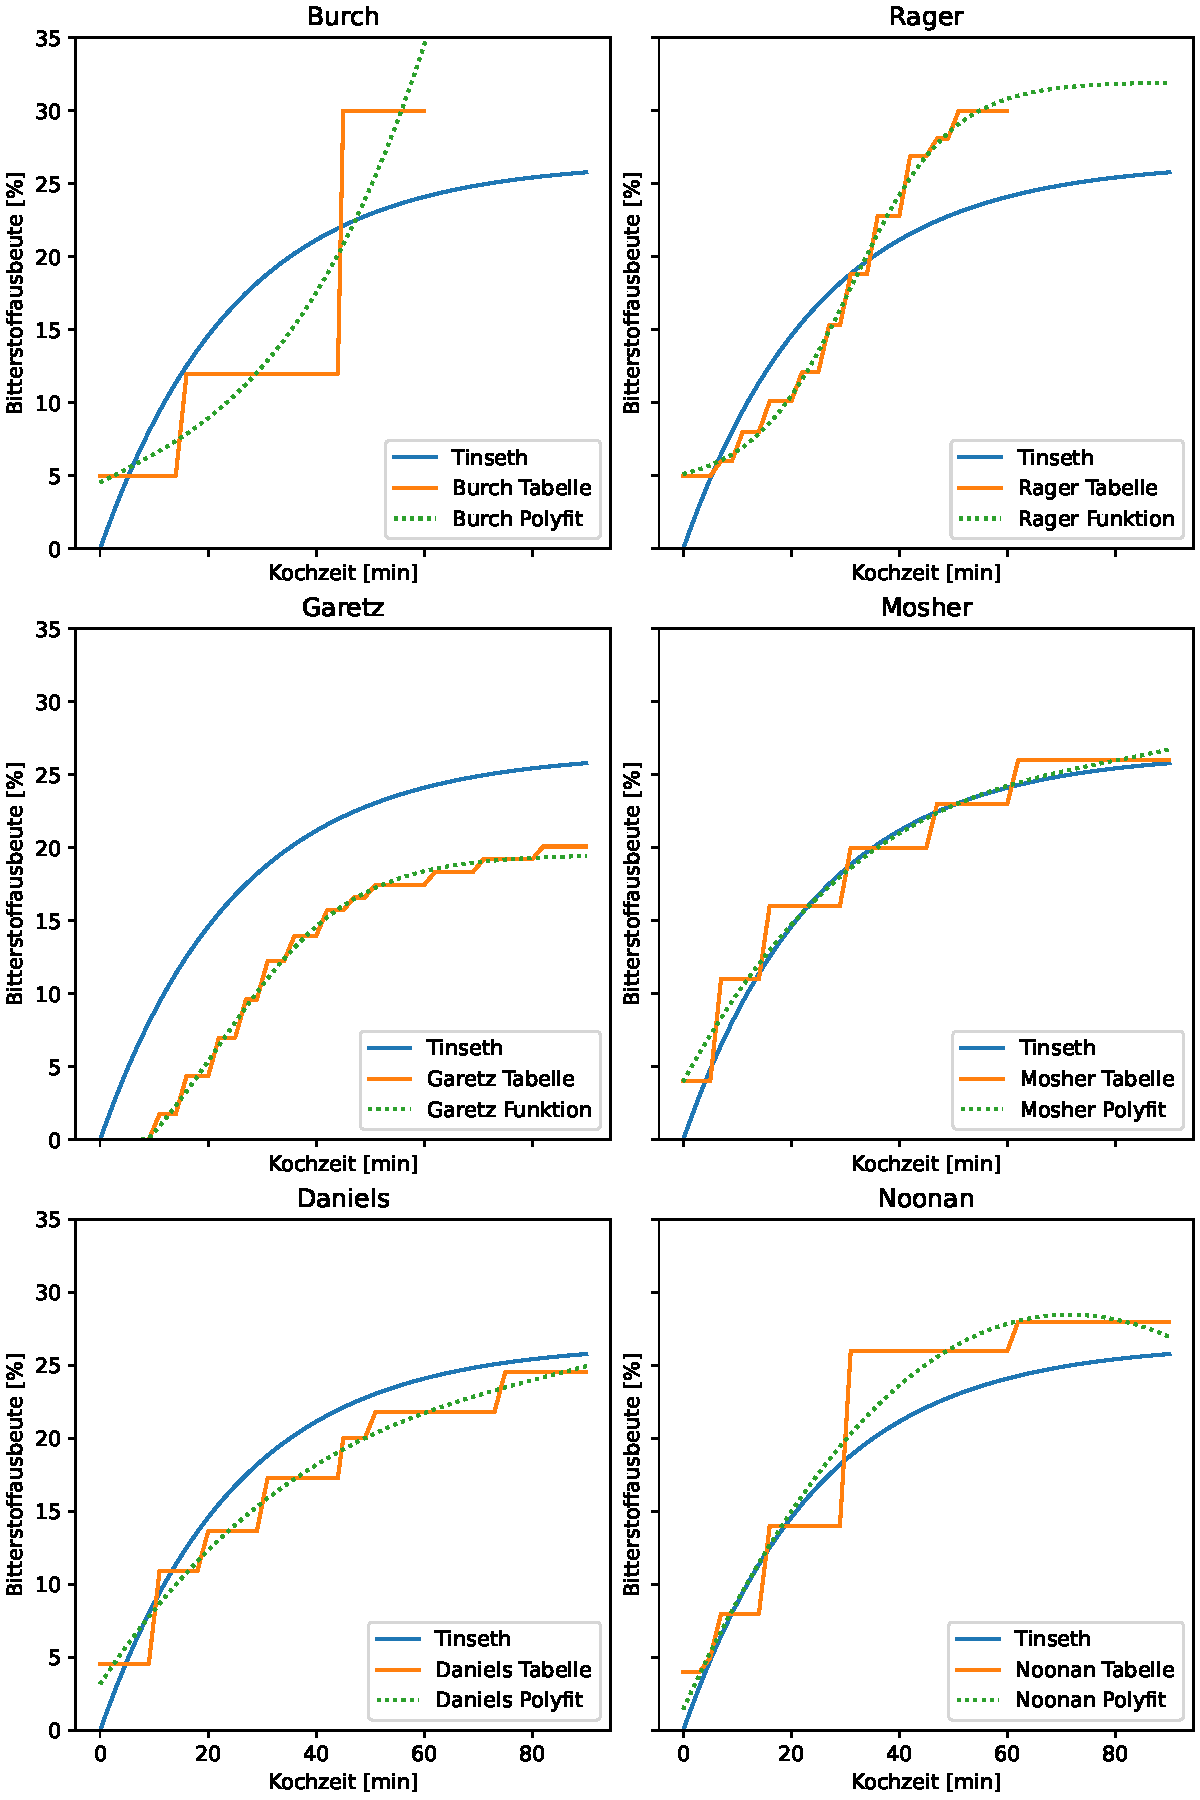
\includegraphics[width=10cm]{graph_utilization.pdf}
\caption{Bitterstoffausbeute bei 10,5 \%w/w Extrakt in Pfvw (Ascher, 2022)}
\label{fig:utilcompare}
\end{figure}

0:47:20-40
IBUS entsprechen nicht perceived bitterness, andere komponenten



1:03:21- time und gravity weil in literatur
die wichtigsten. how much hops 1:04:20

1.06 pale ale 1.07.40
SELBES rezept gescalt, pale ale, ipa, dipa. ctz, cent cascade
20-43 31,8 mit beersmith berechnet

1:08:00 boil vigor, pellets nicht ausgelegt, nie daten genutzt die pellets
pellets waren nicht von gutre qualität 1:09

1:09:38 58
38, 66
dipa 57,9 l 44 71
1:11:00

1:11:35 within 10 % genauigkeit wenn glück, +30
konsistent, sensorisches eindruck korrelieren
1:12:20

1:18:10
protein level 
\parencite{Beechum2017a}

BSHB

11:10--11:14
easily reliable calculate AA Percent

12:00--12:10
11-30% alpha util

20:55-22:00
From Daten nicht herausrechenbar
10 % Genauigkeit
Nicht einmal genau welche alpha der Hopfen weil nur ein eine geringe 
Probe davon.

22:05-23
within 10 ibu
konsistenz ist wichtiger, feinadjustment, nummer nicht,
korrelation zwischen nummer aus gleichung und sensorischem eindruck
\parencite{Smith2011}

Die Beträge der geschätzten
Bitterstoffausbeute scheinen insgesamt zu gering zu sein \parencite{Jones1995}.

Die Beträge
der berechneten Bitterstoffausbeute scheinen insgesamt zu hoch zu sein \parencite{Jones1995}.

\parencite[65]{Hall1997}
Kochbeginn, mitte kochzeit und Ende, Stopfen
45.5
RAGER  57.82
%GARETZ 24.12
MOSHER 35.65
TINSETH  47.54
NOONAN 53.21
DANIELS 46.51

\parencite[65\psqq]{Beechum2017}
Here’s our recommendation: ignore the
number as “concrete reality.” No calcula-
tion is ever going to be perfect for you.
Unless you take the time to dial in your
process, analyze your beers, and create
your own utilization curves, the number
will always be a bit of a lie. Instead, treat it
as a squishy imprecise landmark that only
has meaning for you.
Learn what calculated IBU values of 15,
30, 50, 70, and so on mean to your taste
buds when brewed on your equipment.
Use those landmarks to hit what you want
to taste. That’s the only value to the num-
ber, because, frankly, the number itself is
fairly taste-free.

\parencite{Bonham2001}
Kochzeit , Hopfen bit bekannter Alphasäure und gleicher Brauverfahren
Korrigiert OG
ASBC Mittelwert, 33 Bier: 62.1, 80\% innerhalb einer Abweichung von 15\%, 50\% innerhalb
von  bis 20 Abweichung

Rager: 53.5
Burch: 45.6
Garetz: 41
Mosher: 61
Tinseth: 48
Daniels: 67.9
Noonan: 56.9

\parencite[65]{Beechum2017}
we think the “undershoot” is due to the
rapid chilling procedures that are more
common today than they were during the
formulae’s development.
Well,
one is that there’s probably more work
to be done to figure out how the
numbers change with different chill-
ing regimes, kettle geometry, and boil
vigor.

Well,
one is that there’s probably more work
to be done to figure out how the
numbers change with different chill-
ing regimes, kettle geometry, and boil
vigor.



\subsection*{Aktuelle Ansätze}

\subsubsection*{Wolf (2012)}

„\href{https://www.maischemalzundmehr.de/index.php?inhaltmitte=toolsiburechner}{Maische, Malz und Mehr}“

die Nachisomerisierungzeit (Zeit zwischen Kochende und Whirlpool) wird zur Kochzeit jeder Hopfengabe hinzugerechnet, allerdings entsprechenend ihrer Dauer und der Geschwindigkeit der Abkühlung mit einem niedrigeren Wert gegenüber der regulären Kochzeit (siehe Theorieteil) 

bei Verwendung von Hopfenpellets wird gegenüber Hopfendolden eine 10% höhere Hopfenausnutzung angenommen
Da die Tinseth-Formel auf Experimenten mit Hopfendolden basiert, wird bei der Verwendung von Hopfenpellets die Hopfenausnutzung mit dem Faktor 1.1 nach oben korrigiert, während bei Verwendung von Hopfendolden nicht korrigiert wird. 

Weiterhin hat Glenn Tinseth seine Formel mit Hopfengaben direkt zu Kochbeginn entwickelt. Durch Ausscheidungen mit dem Würzebruch gehen der Würze jedoch eine gewisse Menge an Bitterstoffen verloren. Der IBU-Rechner ehöht die Hopfenausnutzung bei Gaben nach dem Würzebruch um den Faktor 1.1 gegenüber der Tinseth-Formel. Bei Vorderwürzehopfung bzw. bei Hopfengaben zu Kochbeginn gilt die Tinseth-Formel unverändert. 

bei Hopfengaben nach dem Würzebruch (>15 min nach Kochbeginn, d.h. Gesamtkochzeit minus individuelle Hopfenkochzeit > 15) wird eine 10% höhere Hopfenausnutzung angenommen 

In der Zeit zwischen Kochende und Kühlschlange werden weiterhin alpha-Säuren zu iso-alpha-Säuren isomerisiert. Diese Nachisomerisierung wird von der Tinseth-Formel nicht berücksichtigt. Da sie bei Temperaturen <100°C stattfindet, verläuft sie nicht so schnell wie die reguläre Isomerisierung während des Hopfenkochens. Je niedriger die Temperatur, desto langsamer. Die Nachisomerisierung kann mit dem IBU-Rechner jedoch abgeschätzt werden. Dazu wird die Nachisomerisierungszeit zur Würzekochzeit jeder Hopfengabe hinzugerechnet, allerdings entsprechenend ihrer Dauer und der Geschwindigkeit der Abkühlung der Würze mit einem niedrigeren Wert gegenüber der regulären Kochzeit. Dabei wird davon ausgegangen, dass sich die Geschwindigkeit der Isomerisierung alle 10°C unter 100°C halbiert. Diese Abhängigkeit kann mit einem Faktor ausgedrückt werden, welcher bei 100°C daher 1.0, bei 90°C 0.5 und bei 80°C 0.25 usw. entspricht. über eine Regression kann er rechnerisch auch wie folgt ermittelt werden: 

%Isomerisierungsgeschwindigkeitsfaktor = 0.001 x e^0.069 x Temperatur

Mit der Nachisomerisierungszeit multipliziert ergibt dieser Wert die Effektive Kochzeit während der Nachisomerisierung. Bei einer Nachisomerisierung von 30 min und einer Temperatur von 90°C, entspricht die Zeit der Nachisomerisierung effektiv einer Kochzeit von nur 15 min %(Effektive Kochzeit = 30 min x 0.001 x e^0.069 x 90 = 15 min). In der Realität läuft die Nachisomerisierung allerdings nicht bei einer konstanten Temperatur ab. Die Würze kühlt sich in der Nachisomerisierungszeit ausgehend von ca. 100°C kontinuierlich ab. In dieser Abkühlungsphase verringert sich natürlich der Isomerisierungsgeschwindigkeitsfaktor permanent. Messen wir die Temperatur am Ende der Nachisomerisierungszeit, können wir den Isomerisierungsgeschwindigkeitsfaktor allerdings über den Temperaturbereich der Nachisomerisierung (100°C bis Temperatur am Ende der Nachisomerisierung) integrieren: 

%Gleichung 3: Integrierter Isomerisierungsgeschwindigkeitsfaktor = 0.046 e^(0.031 x Temperatur am Ende der Nachisomerisierung). 

Dieser Integrierte Isomerisierungsgeschwindigkeitsfaktor ist dann der Wert, welcher mit der Nachisomerisierungszeit multipliziert die Zeit ergibt, welche im IBU-Rechner zur regulären Kochzeit hinzugerechnet wird. So werden z.B. bei einer Nachisomerisierungszeit von 30 min, während der die Würze auf 80°C abkühlt (errechneter Integrierter Isomerisierungsgeschwindigkeitsfaktor = 0.53), zu jeder Hopfengabe 16 min (30 min x 0.53 = 16 min) zusätzliche Kochzeit hinzugerechnet. Insbesonder bei reichlichen Hopfengaben gegen Kochende, d.h. wenn der Hopfen noch nicht "ausgelutscht" ist, hat die Nachisomerisierung einen enormen Einfluss auf die Gesamtbittere. 

Bereits seit 2012

\parencite{Wolf2022}

\subsubsection*{Hosom – mIBU (2015)}

\url{https://jphosom.github.io/alchemyoverlord}

\parencite{Hosom2015}

\subsubsection*{Novotný (2016)}

\url{https://www.diversity.beer/2018/02/ibu-spreadsheet-english-version.html}
\parencite{Novotny2016}
\parencite{Novotny2018}

\subsubsection*{Smith (2019)}

Zur Berechnung der Bitterstoffausbeute im Whirlpool wendet \citeauthor{Smith2019}
einen von der Temperatur abhängigen, durch \autoref{eq:smithkfwp} definierten,
Korrekturfaktor an. Dabei ist für Hopfengabe, die erst während des Whirlpools
erfolgen, die Ausbeute für eine äquivalente Kochzeit zu berechnen und dann der
Korrekturfaktor anzuwenden. Bei Hopfengaben, die bereits vor dem Whirlpool erfolgt
sind, ist berücksichtigen, dass bereits ein Teil Alphasäuren isomerisiert wurde.
Der verbleibende nicht isomerisierte Säuregehalt ist die Basis für weitere
Berechnungen. \parencite{Smith2019}

\begin{equation}
\mathit{F}_{\mathit{WP}} = 2,39 \cdot 10^{11} \cdot e^{\left(\frac{-9773}{\text{Whirlpool-Temperatur}\:[K]} \right)}
\label{eq:smithkfwp}
\end{equation}

\subsubsection*{Hosom – SMPH (2021)}

\parencite{Hosom2021}

\section*{Berechnungsbespiel}

\section*{Zusammenfassung}

\parencite{Janish2019}
\parencite{Hieronymus2012}
\parencite{Nottebohm2020}
\parencite{Pyle1995}
\parencite{Justus2018}
\parencite{Parkin2017}
\parencite{Bishop1964}
\parencite{Nickerson1979}
\parencite{Calado2019}
\parencite{Weiss2019}

\parencite{Bruecklmeier2017}
\parencite{Bruecklmeier2018}


\printbibliography[title=Quellen]

\end{document}